\section{Dimension three: obstruction to preservation}\label{sec:obstruction}
For $k=3$ the inclusion $\Lambda\subseteq\Lambda'$ no longer implies $U(\Lambda,Q)\subseteq U(\Lambda',Q)$. \Cref{thm:evensum} already gives an infinite family with rectangular target $\bigoplus o_i\Z$. This section shows that the failure does not depend on the target having a coordinate on which it is ``free'', and gives the exact structure of the failing cells.

\subsection{Dilation invariance}
\begin{theorem}[diagonal dilation]\label{thm:D1}
Let $D=\mathrm{diag}(t_1,\dots,t_k)$ with $t_i$ positive integers and $M$ a lattice. Then $\Gr(DM)=D\,\Gr(M)$, $F(DM,DQ)=D\,F(M,Q)$, cells go to cells, $U(D\Lambda,DQ)=D\,U(\Lambda,Q)$, and
\[
U(\Lambda,Q)\subseteq U(\Lambda',Q)\iff U(D\Lambda,DQ)\subseteq U(D\Lambda',DQ).
\]
\end{theorem}
\prov{CW-0507}{P5-D1}{PROVED}{FULL}
\begin{proof}
$D:M\to DM$ is a bijection of lattices and $Dw\cm Dv\iff w\cm v$ (signs agree and $|t_iw_i|\le|t_iv_i|\iff|w_i|\le|v_i|$), so $D$ preserves the conformal order, hence Graver sets, independence, and the corner condition; it maps $M\cap[0,Q]$ onto $DM\cap[0,DQ]$ and $0$ to $0$. Cells are affine images of cubes. \qedhere
\end{proof}
Dilation changes the axis orders: the property ``$e_c\notin\Lambda'$'' is not dilation invariant, and a failure with a free coordinate becomes a failure in which every axis order is $\ge2$.

\subsection{A failure without free coordinate, and its dilation family}
\begin{theorem}[failure with no free coordinate]\label{thm:C1}
Let $E_3=\{z\in\Z^3:\sum z_i\text{ even}\}$, $\Lambda=2E_3\subseteq\Lambda'=2\Z^3$ (axis orders $(2,2,2)$: no $e_i$ lies in $\Lambda'$) and $Q=(2,4,2)$. Then $U(\Lambda,Q)\not\subseteq U(\Lambda',Q)$.
\end{theorem}
\prov{CW-0508}{P5-C1}{PROVED}{FULL}
\begin{proof}
$\Gr(2E_3)=2\,\Gr(E_3)$ (\cref{thm:D1} and \cref{prop:E25}). Let $g=(0,2,-2)=2(0,1,-1)$, $h=(2,-2,0)=2(1,-1,0)$, $u=(0,2,2)$. The corners $(0,2,2),(0,4,0),(2,0,2),(2,2,0)$ are nonzero points of $2E_3\cap Q$, so $c=\Pil(u;g,h)$ is a $2$-cell of $U(\Lambda,Q)$. The point $p=u+\tfrac16g+\tfrac13h=(\tfrac23,\tfrac53,\tfrac53)$ lies in $c$. In $U(2\Z^3,Q)$ the Graver vectors are $\pm2e_i$, so every cell is $\Pil(c';2e_i,i\in I)$ with $c'\in2\Z^3$. A cell containing $p$ must, for each coordinate $i$ with $0<p_i<2$ (all three do), use the generator $2e_i$ with base coordinate $0$; that cell is $[0,2]^3$, whose corner $0$ is excluded. So $p\notin U(\Lambda',Q)$. \qedhere
\end{proof}
\begin{figure}[tbp]\centering
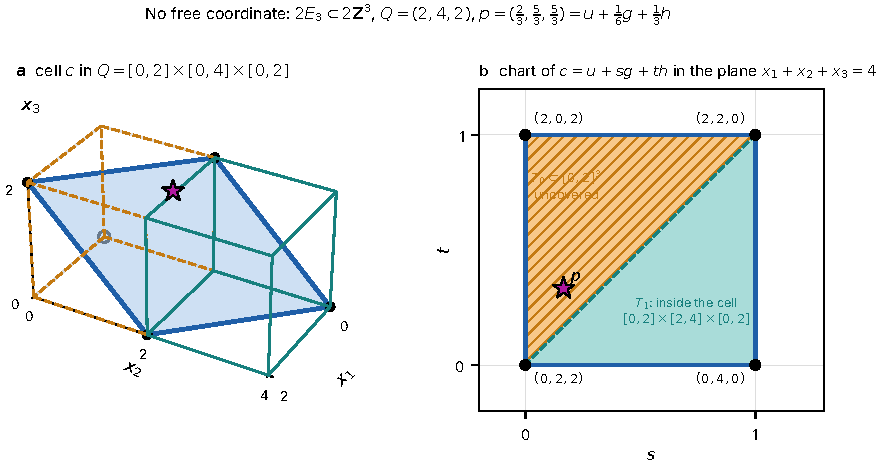
\includegraphics[width=0.98\textwidth]{fig09_noncontainment_3d}
\caption{Three-dimensional non-containment (\cref{thm:C1}; $\Lambda=2E_3\subset\Lambda'=2\Z^3$, $Q=(2,4,2)$; \emph{exact computation}). (a)~The $2$-cell $c=\Pil((0,2,2);(0,2,-2),(2,-2,0))$ of $\Kabs(2E_3,Q)$ in the box $[0,2]\times[0,4]\times[0,2]$ with its four corners $(0,2,2)$, $(0,4,0)$, $(2,0,2)$, $(2,2,0)$. (b)~The chart $c=u+sg+th$, $(s,t)\in[0,1]^2$, in the plane $x_1+x_2+x_3=4$: the part $T_0$ of $c$ inside the cube $[0,2]^3$ (light orange) is not covered by any cell of $\Kabs(2\Z^3,Q)$, whereas the part $T_1$ (outside that cube) is. The star is the witness $p=(\frac23,\frac53,\frac53)=u+\frac16g+\frac13h\in T_0$, in $c$ but in no cell of $\Kabs(2\Z^3,Q)$ (exact enumeration); hence $U(2E_3,Q)\not\subseteq U(2\Z^3,Q)$.}\label{fig:noncontain}
\end{figure}
\begin{corollary}[infinite family]\label{cor:C2}
If $(\Lambda,\Lambda',Q)$ fails (i.e.\ $U(\Lambda,Q)\not\subseteq U(\Lambda',Q)$) then so does every dilation $(D\Lambda,D\Lambda',DQ)$. In particular every failing triple with a free coordinate, such as the scaled $E_3\subset\Z^3$, $Q=(1,2,1)$, $p=(\tfrac13,\tfrac56,\tfrac56)$, generates failing triples all of whose axis orders are $\ge2$.
\end{corollary}
\prov{CW-0509}{P5-C2}{PROVED}{FULL}
\begin{proof}
\Cref{thm:D1}. \qedhere
\end{proof}
\begin{figure}[tbp]\centering
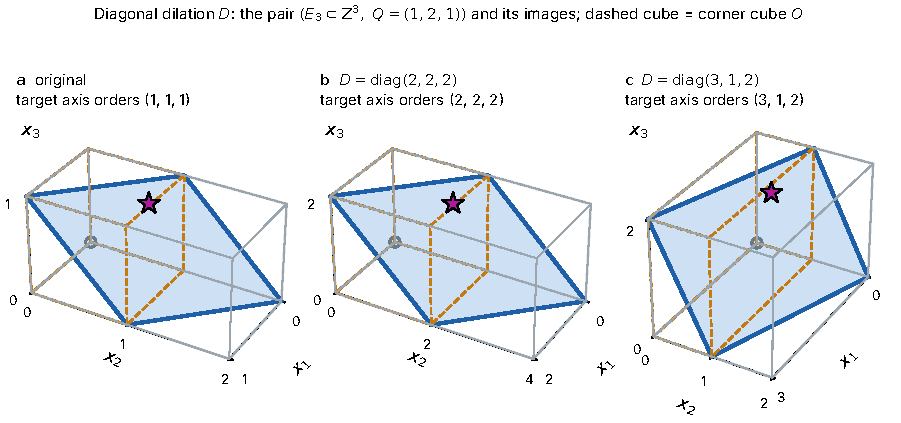
\includegraphics[width=0.98\textwidth]{fig10_dilation}
\caption{Diagonal dilation preserves failure (\cref{thm:D1,cor:C2}; \emph{exact computation}). The failing pair $(E_3\subset\Z^3,Q=(1,2,1))$ with its witness $(\frac13,\frac56,\frac56)$ (a) and two dilations: $D=\mathrm{diag}(2,2,2)$ giving $(2E_3\subset2\Z^3,(2,4,2))$ with witness $(\frac23,\frac53,\frac53)$ (b) --- the configuration of \cref{fig:noncontain} --- and $D=\mathrm{diag}(3,1,2)$ giving the box $(3,2,2)$ with witness $(1,\frac56,\frac53)$ (c). In each panel the transformed box, the cell and the transformed corner cube (dashed) are drawn; the target axis orders are $(1,1,1)$, $(2,2,2)$ and $(3,1,2)$, so in (a) every coordinate is free, in (b) none is, and in (c) only $x_2$ is. Failure was verified exactly in all three cases.}\label{fig:dilation}
\end{figure}
\begin{remark}[relation to the corner-cube theorem]
Theorem~\ref{thm:C1} is the instance $o=(2,2,2)$ of \cref{thm:evensum}: the scaled source lattice is $E_3$, the scaled box is $(1,2,1)$ with maximum $2$, and the scaled point is $(\tfrac13,\tfrac56,\tfrac56)\in O$. The target $2\Z^3$ is rectangular in the sense of \cref{sec:corner}; the release derived the same example independently and emphasises ``no free coordinate'' because the earlier three-dimensional conjecture was formulated in those terms. (The identification is derived here from the two cited theorems and the scaling invariance; it is an elementary observation.) The recorded $57$ lattice-level failures with a free coordinate are finite-exact data of the releases and are not used.
\end{remark}

\subsection{A target that is not split in any coordinate}
\begin{proposition}[FINITE-EXACT; body-centred target]\label{prop:C3}
Let $\Lambda=2E_3$, $\Lambda'=\mathrm{BCC}=\{z\in\Z^3:z_1\equiv z_2\equiv z_3\ (2)\}$ (index $4$, axis orders $(2,2,2)$, not split in any coordinate: $\Lambda'\ne(\Lambda'\cap\{z_i=0\})\oplus(\Lambda'\cap\R e_i)$ for each $i$) and $Q=(2,4,2)$. Then $\Lambda\subseteq\Lambda'$ and $U(\Lambda,Q)\not\subseteq U(\Lambda',Q)$; the cell $c$ of \cref{thm:C1} contains the point $(\tfrac56,\tfrac53,\tfrac32)=u+\tfrac14g+\tfrac5{12}h$, which is not in $U(\mathrm{BCC},Q)$. The same source cell is contained in $U(E_3,Q)$ (release; also sampled at $49$ interior points here).
\end{proposition}
\prov{CW-0510}{P5-C3}{FINITE-EXACT}{FINITE}
\noindent\emph{Evidence and scope.} The statement is a finite exact computation: for $Q=(2,4,2)$, $\Kabs(\mathrm{BCC},Q)$ has $13$ vertices, $33$ edges, $17$ squares and one cube, and the point lies in no cell. The release certified this by three routes (an engine with an independent certificate checker, a mini brute-force implementation, and the preregistered pinned engine); it was reproduced here with a fourth, independent exact implementation (\texttt{scripts/run\_exact\_checks.py}). Non-splitness of BCC: for each $i$, $\Lambda'\cap\{z_i=0\}=2\Z^2$ and $\Lambda'\cap\R e_i=2\Z e_i$, whose direct sum has index $8$ in $\Z^3$, while $[\Z^3:\Lambda']=4$; so $\Lambda'$ is not that direct sum. The release also records failure for $\Lambda'=E_2\times2\Z$ (split in one coordinate), cited. \textbf{Consequence:} neither ``no free coordinate'' nor even ``no split coordinate'' implies preservation; the $3$-dimensional conjecture of the earlier assessment ($\Lambda\subseteq\Lambda'\subseteq\Z^3$, $e_1,e_2,e_3\notin\Lambda'\Rightarrow U\subseteq U'$) is false, by \cref{thm:C1} already.

\begin{figure}[tbp]\centering
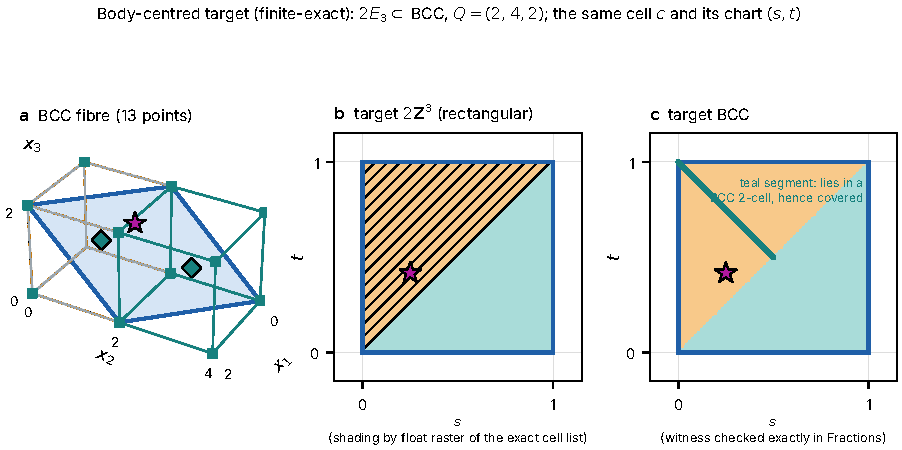
\includegraphics[width=0.98\textwidth]{fig11_bcc}
\caption{The body-centred target (\cref{prop:C3}; FINITE-EXACT for $Q=(2,4,2)$ only). The cell $c$ of \cref{fig:noncontain} and its chart $(s,t)$. (a)~The $13$ points of $F(\mathrm{BCC},Q)$, $\mathrm{BCC}=\{z_1\equiv z_2\equiv z_3\ (2)\}$. (b)~With the rectangular target $2\Z^3$ ($f$-vector $(11,17,8,1)$) the uncovered region is the orange triangle $T_0$ of \cref{fig:noncontain}. (c)~With the BCC target ($f$-vector $(13,33,17,1)$) the uncovered region is $T_0$ minus a teal segment, which lies in a BCC $2$-cell and is therefore covered; but the exact witness $p=(\frac56,\frac53,\frac32)$ (chart coordinates $(\frac14,\frac5{12})$, star) lies in no cell of $\Kabs(\mathrm{BCC},Q)$. Shading is a floating-point raster (uncovered fractions $\approx0.497$ and $\approx0.493$ of the chart); the verdict at $p$ is exact. This is a finite-exact example, not a classification of non-split targets.}\label{fig:bcc}
\end{figure}
\subsection{Cells inside a coordinate plane are preserved}
\begin{theorem}\label{thm:F1}
Let $\Lambda\subseteq\Lambda'\subseteq\Z^3$ and let $c$ be a cell of $U(\Lambda,Q)$ contained in a coordinate plane $H=\{x_i=0\}$. Then $c\subseteq U(\Lambda',Q)$. So a failing cell is never in a coordinate plane.
\end{theorem}
\prov{CW-0506}{P5-F1}{PROVED}{FULL}
\begin{proof}
A vector conformally below one in $H$ lies in $H$, so $\Gr(M\cap H)=\Gr(M)\cap H$ for every lattice $M$. Hence $c$ is a cell of the planar pair $\Lambda\cap H\subseteq\Lambda'\cap H$ (both of rank $2$), and \cref{thm:planar} gives $c\subseteq U(\Lambda'\cap H,Q\cap H)$. Cells of $\Lambda'\cap H$ with corners in $F(\Lambda'\cap H)$ are cells of $\Lambda'$ (their generators are Graver in $\Lambda'$ by the same identity), so $U(\Lambda'\cap H,Q\cap H)\subseteq U(\Lambda',Q)$. \qedhere
\end{proof}

\subsection{Finite census (finite-exact)}
\begin{proposition}[FINITE-EXACT; scope as stated]\label{prop:census}
Targets of index $2$--$6$ without a free coordinate ($96$ lattices), sources of index $2$--$5$ ($8{,}256$ pairs), all hard cells with bounding box $\le Q_{\max}=(\min(3k_c,12))_c$: $24{,}178$ hard cells ($6{,}825$ squares, $17{,}353$ cubes), each tested against its own worst box. $192$ hard cells fail; the failing targets are $19$ of the $96$: all $12$ split targets and $7$ of $84$ non-split targets (BCC and six of index $6$). The remaining $77$ non-split targets (including $E_3$ and every target of index $3$ and $5$) have no failure among $19{,}794$ hard cells. An extended run (sources of index $6$--$9$ in the $18$ clean targets of index $\le4$) found $19{,}877$ hard cells and no failure.
\end{proposition}
\prov{CW-0512}{census}{FINITE-EXACT}{FINITE}
\noindent These numbers are samples, not a classification theorem, and the release states explicitly that its earlier remark ``no zero-vertex decomposition occurred'' was an artefact of box scope. They are included only to indicate that preservation for non-split targets is genuinely dependent on the target lattice; the question of which non-split targets preserve $U$ is open (\cref{sec:open}).
